\pagebreak
\chapter{Continuous Integration}
Dieses Kapitel beschäftigt sich mit einem der beiden Hauptthemen, nämlich Continuous Integration. Dabei möchte ich mich diesem Thema zunächst durch eine genaue Begriffsbestimmung nähern, wobei auch eine Abgrenzung zu anderen, ähnlichen Begriffen eine wichtige Rolle spielt. Im weiteren Verlauf sollen dann noch der Einsatz von Tools zur Unterstützung sowie die Gründe zum Einsatz dieser Methodik näher beleuchtet werden.\\
\section{Begriffsklärung}
Den Einstieg soll eine kurze Beschreibung von Martin Fowler bilden, er gilt als der gesitige Vater von Continuous Integration und wird mit diesem Artikel in vielen anderen Abhandlungen zu dem Thema zitiert:
\begin{center}
	\textit{
	Continuous Integration is a software development practice where members of a team integrate their work frequently, usually each person integrates at least daily - leading to multiple integrations per day. Each integration is verified by an automated build (including test) to detect integration errors as quickly as possible} \cite{fowler-CI}
\end{center}
Es geht hier also um das kollaborative Arbeiten in einem Team, insbesondere das Integrieren von Code in eine gemeinsame Code-Basis. Das heißt ferner, dass es eine Methodik ist die für einen einzelnen Entwickler kaum Bedeutung hat. Das ist auch einleuchtend, denn seinen eigenen Code in eben diesen zu integrieren, macht kaum Sinn. \\
Ferner sollte dies sehr oft passieren, am besten mehrmals täglich. Auch das ist eine sehr sinnvolle Daumenregel. Wenn man zu lange seinen Code nicht in die gemeinsame Code-Basis integriert, so besteht die Gefahr, dass man zu weit weg ist davon und dadurch immense Aufwände entstehen. Dann wird aus dem Integrieren einer eigentlich keinen Änderung eine umfassende Merge\footnote{Mergen bezeichnet das Vergleichen mehrerer Änderungen an einer Quelldatei und das Zusammenführen ("`mergen"') dieser Änderungen. vgl.:\url{https://de.wikipedia.org/wiki/Merge}}-Session.\\
Der dritte Teil der vorliegenden Beschreibung geht darauf ein, wie man den Nachweis erbringen kann, dass die Integration erfolgreich war. Dafür soll es automatisierte (und dadurch auch standardisierte) Builds geben. Diese Builds erzeugen zunächst aus dem menschenlesbaren Code den von Maschinen ausführbaren Code sowie dazu gehörige Tests in verschiedenem Detailgrad. Martin Fowler gibt in seienr Beschreibung auch an, dass die Tests mit zu diesem automatisierten Builds gehören. Hierbei muss man auf eine sinnvolle Testtiefe achten. Wenn man die Test-Pyramide\footnote{Dabei handelt es sich um eine Darstellung der unterschiedlichen Testtypen in hierarchischer Form, wobei von unten nach oben die Geschwindigkeit abnimmt und die Kosten zunehmen. vgl.:\cite{fowler-Testpyramid}} zu Rate zieht, muss man darauf achten, dass alle Tests fertig sind bevor der nächste Entwickler sein Änderungen in die Code-Basis integriert. Deshalb ist es eventuell am Besten, wenn man während des initialen Builds nur Unittests ausführt, und ein möglicherweise nur einmal am Tag laufender Build dann detailierter testet.\\
Um diese Beschreibung der Kernpunkte von Continuous Integration auf eine breitere Basis zu stellen, möchte ich noch eine zweite Quelle nutzen, um von einem anderen Blickwinkel auf das Thema zu blicken.
\begin{center}
	\textit{
The practice of continuous integration represents a fundamental shift\\ in the process of building software. It takes integration, commonly\\
an infrequent and painful exercise, and makes it a simple, core part\\ of a developer’s daily activities. Integrating continuously makes\\ integration a part of the natural rhythm of coding, an integral part\\ of the test-code-refactor cycle. Continuous integration is about\\ progressing steadily forward by taking small steps.}\\ \cite{10.1007/978-3-540-24853-8_8}
\end{center}
Der Autor dieses Konferenzbeitrags ist R. Owen Rogers. Er arbeitet bei Thoughtworks, derselben Firma bei der auch Martin Fowler arbeitet. Er stammt von einer Konferenz aus dem Jahr 2004, also zeitlich zwischen der initialen Version über CI\footnote{Ab hier werde ich CI als Abkürzung für "`Continuous Integration"' verwenden. Diese Abkürzung ist auch im Abkürzungsverzeichnis zu finden.} seiner aktuellen Version aus dem Jahr 2006.\\
Es wird dabei eher der Fokus auf die Auswirkungen von Continuous Integration auf die Softwareentwicklung und der Einfluss auf die Qualität von Software gelegt. Er geht dabei vor allem darauf ein, dass das häufige Integrieren der zentrale Teile dieses Konzepts ist. Das deckt sich mit der oben vorgestellten Sichtweise von Martin Fowler. Des weiteren setzt er den Ansatz in den Kontext von "`test-code-refactor"', und geht damit auch auf einen anderen bereits vorgestellten Aspekt ein, nämlich das Überprüfen des Erfolgs der Integration. Der Anteil, dass es eine Praktik ist, die hauptsächlich in Teams Sinn macht, ist eher implizit enthalten in diesem Text und wird nicht extra erwähnt.\\
Er deckt sich damit mit der Sichtweise von Martin Fowler, und beleuchtet das Thema einfach nur aus einem anderen, eher anwendungsbezogenen Blickwinkel. Das ist auch nachvollziehbar, da es sich hier nicht um eine theoretische Abhandlung handelt sondern einen Konferenzbeitrag, der an Anwender dieser Technik gerichtet war.\\

Zusammenfassend bleibt zu sagen dass mit Continuous Integration die Zusammenarbeit eines Entwicklerteams an einer gemeinsamen Code-Basis verbessert werden soll. Dies soll geschehen durch kontinuierliches Zusammenführen der Änderungen aller Beteiligten und das automatisierte Prüfen des Ergebnisses.
\subsection{Abgrenzung zu anderen Begriffen}
Es gibt einige Begriffe die Continuous Integration sehr ähnlich sind. Dieser Abschnitt soll genauer umreißen, wo der Unterschied ist und was sie vielleicht gemeinsam haben.
\begin{itemize}
	\item\textbf{Continuous Delivery}\\
	Auch hier hat Martin Fowler eine zusammenfassende Definition geliefert:
\begin{center}
	\textit{
	You achieve continuous delivery by continuously integrating the \\software done by the development team, building executables, and\\ running automated tests on those executables to detect problems. \\Furthermore you push the executables into increasingly production-like \\environments to ensure the software will work in production. To do \\this you use a DeploymentPipeline.}\\ \cite{fowler-CD}
\end{center}
	Bei Continuous Delivery (CD\footnote{Ab hier werde ich CD als Abkürzung für "`Continuous Delivery"' verwenden. Diese Abkürzung ist auch im Abkürzungsverzeichnis zu finden.}) wird der Gedanke von Continuous Integration aufgegriffen, und weiterentwickelt. Während Continuous Integration sich komplett in der Entwicklung bewegt, umfasst Continuous Delivery auch Schritte bis hin zum Kunden. Es werden weitere Schritte wie das Paketieren als Deliverable (z.B. Erstellen eines Setups) und das Deployment (z.B. Bereitstellen als Download oder Einstellen in einen AppStore) betrachtet. Das Ziel dessen ist, dass das Ergebnis der Entwicklung zu jedem Zeitpunkt zum Kunden geschickt werden könnte.\\
	\item\textbf{Continuous Deployment}\\
	Hier beziehe ich mich auf den Abstract eines Konferenzbeitrages von Helena Holmström Olsson
	\begin{center}
		\textit{
		The concept of continuous deployment, i.e. the ability to deliver software functionality frequently to customers \textelp{}}\\
		\cite{olsson2012climbing}
	\end{center}
	Continuous Deployment bringt das CI-Konzept zwei Schritte weiter. Nicht nur wird hier wie bei Continuous Delivery in "`Production-like"' Umgebungen installiert sondern sehr häufig (potentiell mit jedem Build) in die Produktion gegeben. Der Unterschied ist hier erstmal nur marginal, aber prinzipiell kann man sagen, dass bei Continuous Delivery festgelegt wird, wann man in die Produktion geht, und bei Continuous Deployment dies laufend passiert. \cite{scrum-overview-ci-cd}. Das heißt aber auch, dass dieses Konzept das am weitesten automatisierte ist mit allen Vor- und Nachteilen.
	
\begin{figure}[h]
  \centering
  \fbox{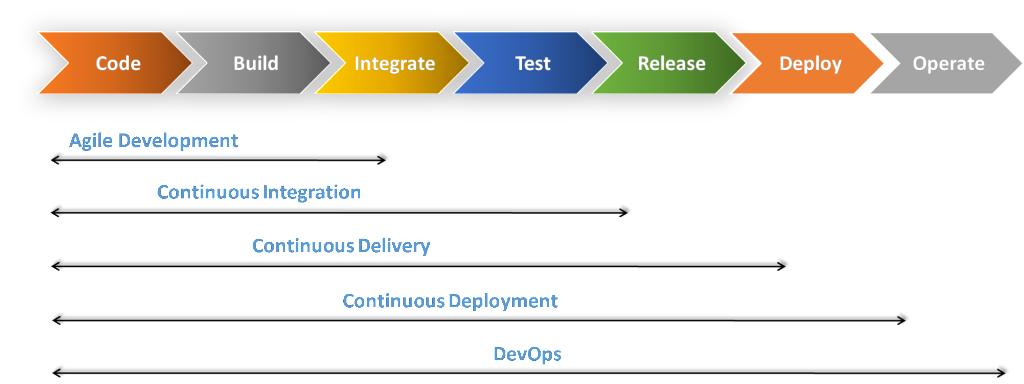
\includegraphics[width=\textwidth]{./Images/ci-cd-image-1024x384.png}}
  \caption{Übersicht über verschiedene Begriffe \cite{Begriff-Overview}}\label{fig:ci-cd-image-1024x384}
\end{figure}
	
\end{itemize}
\section{Ablauf von Continuous Integration}
Da in der Beschreibung von CI die Rede ist vom Integrieren von Code Änderungen, muss es auch irgendwie eine gemeinsame Basis geben, in die diese Änderungen einfließen. Eine solche gemeinsame Basis ist ein sogenanntes Source-Control-Management-System (SCM\footnote{Ab hier werde ich SCM als Abkürzung für "`Source Control Management"' verwenden. Diese Abkürzung ist auch im Abkürzungsverzeichnis zu finden.}). Dabei handelt es sich um ein System, in dem Änderungen an einer Datei, oder der Struktur der Dateien, nachvollziehbar gemacht werden, und man verschiedene Stände abrufen kann.(vgl. \cite{fowler-CI}) Es gibt dazu verschiedene Konzepte, entweder eine zentrale Stelle an der alle Dateien inklusive Historie verwaltet werden, oder verteilte Systeme, bei der es keine ausgezeichnete zentrale Instanz gibt.\\
\begin{figure}[h]
  \centering
  \fbox{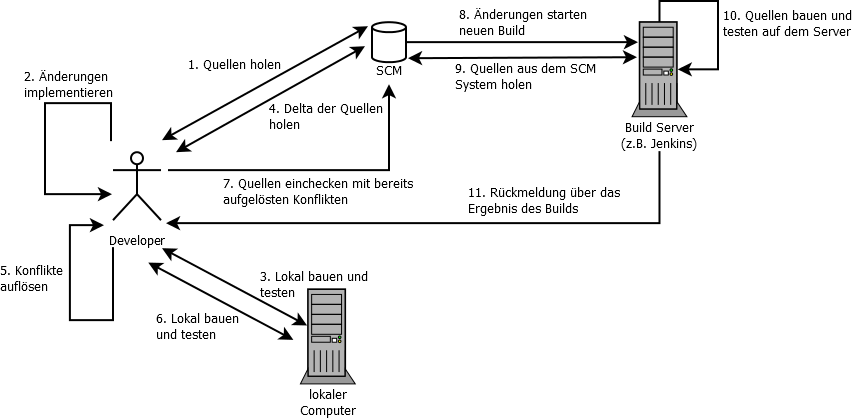
\includegraphics[width=\textwidth]{./Images/Schema-aufbau.png}}
  \caption{Schematischer Ablauf von CI}\label{fig:Schema-aufbau}
\end{figure}
\begin{enumerate}
	\item \textbf{Get Sources}\\% 1
		Die Arbeit des Entwicklers basiert auf dem aktuellen Stand der Quellen aus dem SCM. Deshalb holt er sich zunächst diesen auf seinen lokalen Computer, um seine Arbeit zu beginnen.
		\item \textbf{Implement the Changes to the Code}\\% 2
		Der Entwickler folgt diesem Prozess aus einem bestimmten Grund, nächlich entweder ein neues Feature zu implementieren oder bekannte Fehler in der Software zu beheben. Dies geschieht in diesem Schritt. Der Entwickler führt die ihm übertragenen Aufgaben aus. Dabei wird bei CI besonders Wert auf Tests gelegt. Dies ist mittlerweile zum Quasistandard in der Sotwareentwicklung geworden, und folgt vom schematischen Aufbau her der Testpyramide, wie sie in (\cite{fowler-Testpyramid}) beschrieben wird.
		\item \textbf{Build locally including tests}\\% 3
		Der vorhergehende Schritt hat sich komplett auf das Implementieren von Code bzw. Codeänderungen sowie das Implementieren und Ändern von Tests beschränkt. Diese müssen auch noch auch Fehlerfreiheit überprüft werden, bevor man sie in das SCM einfügt. Die erste Kontrollinstanz ist nun der automatisierte Build auf der Entwicklermaschine. Darunter versteht man das Kompilieren und Linken der Quellen sowie das Ausführen der zuvor geschriebenen automatisierten Tests. Hierbei beschränkt man sich zumeist auf UnitTests.
		\item \textbf{Get Source Code Delta}\\% 4
		Während der Entwickler seinen Auftrag ausgeführt hat, haben einige seiner Kollegen bereits ihre Arbeit vollendet. Deshalb muss er nun den aktuellen ("`top-level"') Stand holen, weil es sonst zum Beispiel passieren könnte, dass er Änderungen überschreibt bzw. es Konflikte gibt beim Hinzufügen, die nicht automatisch aufgelöst werden können.
		\item \textbf{Resolve Conflicts}\\% 5
		Falls der Entwickler nun in die Situation gekommen ist, dass seine lokalen Änderungen mit Änderungen, die bereits im SCM sind in Konflikt stehen, so muss er diese manuell auflösen. Es gibt einige Konflikte die grundsätzlich auch toolunterstützt automatisch auflösbar sind (z.B. Änderung an derselben Datei aber in unterschiedlichen Zeilen), jedoch muss bei manchen Konflikten einfach ein Mensch entscheiden, was der richtige Schritt ist.
		\item \textbf{Build locally including tests}\\% 6
		Der Entwickler muss nun überprüfen ob seine Änderungen noch funktionieren und alle Tests weiterhin fehlerfrei sind. Dies betrifft nun nicht nur seinen eigenen Code sondern auch den der anderen Entwickler. Es ist denkbar, dass seine Änderungen Auswirkungen an anderen Stellen haben. Dabei ist auch er selbst in der Verantwortung, dass der Code-Stand den er später dem SCM hinzufügen möchte funktioniert. Dies geschieht auf seinem lokalen Rechner.		
		\item \textbf{Check-In Source Code with conflicts already resolved}\\% 7
		Nachdem lokal der Code erfolgreich kompilierbar ist, und alle (Unit-)Tests fehlerfrei sind, kann der Entwickler seine Änderungen dem SCM hinzufügen.
		\item \textbf{New Changes trigger Automated Build}\\% 8
		Je nach SCM und Build Server Kombination gibt es mehrere denkbare Ansätze automatisiert nach jedem Check-In von Code einen Build zu triggern. Diese basieren prinzipiell auf einem Observer Pattern\footnote{Ziel des Observer Patterns ist es eine sog. one-to-many Beziehung zwischen Objekten zu definieren, so dass eine Statusänderung eines Objektes all davon abhängigen Objekte benachrichtigt, bzw. automatisch ändert. vgl. auch \cite{hannemann2002design}} entweder mit Push-Notification (Jede Änderung benachrichtigt automatisch alle Subscriber) oder Pull-Notification (Regelmäßiges Nachfragen der Subscriber, ob sich etwas geändert hat). Egal welche der Methoden zum Einsatz kommt, nach dem Hinzufügen der Änderungen wird ein Build gestartet.
		\item \textbf{Get those sources from SCM System}\\% 9
		Der Build Server wurde bisher nur benachrichtigt, es ist aber bisher noch kein Inhalt übertragen worden. Das geschieht in diesem Schritt. Der Einfachheit halber habe ich dabei in \autoref{fig:Schema-aufbau} nur einen einzigen Build Server eingefügt. Prinzipiell gibt es eine Orchestrierung-Instanz und mehrere Build Server. Diese zentrale Instanz koordiniert dabei die Aufgaben und die Server führen diese aus. Im vorliegenden Schaubild ist sowohl die koordinierende Instanz als auch die ausführende auf demselben Server. Die Übertragung findet zur ausführenden Instanz statt, da diese auch den Code kompiliert und testet.
		\item \textbf{Build and Test the Code}\\% 10
		Hier wird, genau wie auch auf dem lokalen Rechner des Entwicklers der Code gebaut und getestet. Der große Vorteil gegenüber den Entwicklerrechnern ist, dass es eine klar definierte Instanz ist. Entwicklerrechner sind sehr heterogen vom Aufbau, da im Laufe der Zeit immer mehr "`HilfsTools"' die das Arbeiten erleichtern hinzukommen. Der Build Server ist anders, denn er hat ein klar definiertes Set von installierten Programmen und installierten Bibliotheken, die zum Erstellen der Kompilate benutzt werden können. Hier fällt zum ersten Mal auf, wenn der Entwickler sich auf etwas verlässt, das nur auf seiner Maschine vorhanden ist. Dazu zählen auch neue Kompilate. Wenn die Source Dateien nicht explizit in das SCM eingefügt wurden bzw. die Anweisung zum Erstellen des Kompilats aus diesen hinzugefügt wurde, funktioniert zwar der lokale Build aber nicht der Server Build. Dies ist das zentrale Quality Gate im CI Prozess und aufgrund des automatisierten Prozesses und der klar definierten Umgebung die Komponente die das größte Vertrauen in das Ergebnis besitzt.
		\item \textbf{Give Feedback about the outcome of the build}\\% 11
		Nachdem der Build fertig ist, muss der Entwickler auch noch auf irgendeine Art und Weise Kenntnis vom Ergebnis erlangen. Entweder wird es auf einer Webseite veröffentlicht, oder er bekommt direkt eine Email mit dem Ergebnis, oder eine Kombination aus beidem. Dies ist wichtig, denn egal wie der Build verlaufen ist, ist es wichtig für die weitere Arbeit. Der schlimmere Fall ist, dass der Build nicht funktioniert hat. Das bedeutet, dass alle anderen Entwickler die sich auf diesen Build stützen blockiert sind in ihrer Arbeit. Es heißt dann also so schnell wie möglich den Grund zu finden und dieses Problem zu beheben. Potentielle Lösung wäre auch, die Änderungen im SCM rückgängig zu machen, damit die anderen Entwickler erst mal ungestört weiter arbeiten können. Im guten Fall, dass der Build erfolgreich war, signalisiert die Benachrichtigung, dass der Entwickler sich nun der nächten Aufgabe widmen kann.
\end{enumerate}
%Ein Entwickler nimmt sich nun den aktuellen Stand aus diesem SCM, und führt seine Arbeit aus. Dabei wird bei CI besonders Wert auf Tests gelegt. Dies ist mittlerweile zum Quasistandard in der Sotwareentwicklung geworden, und folgt vom schematischen Aufbau her der Testpyramide, wie sie in (\cite{fowler-Testpyramid}) beschrieben wird.\\
%Die erste Kontrollinstanz ist nun der automatisierte Build auf der Entwicklermaschine. Darunter versteht man das Kompilieren und Linken der Quellen sowie das Ausführen der zuvor geschriebenen automatisierten Tests. Hierbei beschränkt man sich zumeist auf UnitTests.\\
%Wenn dieser Schritt zufriedenstellend abgeschlossen ist, können die Änderungen zurück in das SCM geführt werden. Dazu holt der Entwickler sich abermals den aktuellen Stand, und löst potentielle Konflikte auf, die entstanden sind, weil andere Entwickler in der Zwischenzeit ihren Stand eingefügt haben. Lokal hat er nun bereits den neuen Stand, den er nun noch einmal lokal baut und testet. Ist dieser lokale Build erfolgreich, fügt er seine Änderungen dem SCM hinzu. An diesem Punkt startet der automatische Prozess der Buildumgebung. Sobald die Änderungen im Source Control sind, wird ein Build getriggert. Der Einfachheit halber habe ich dabei in Abbildung~\ref{fig:Schema-aufbau} nur einen einzigen Build Server eingefügt. Prinzipiell gibt es eine Orchestrierungs-Instanz und mehrere Build Server. Diese zentrale Instanz koordiniert dabei die Aufgaben und die Server führen diese aus.
\section{Gründe Continuous Integration einzusetzen}
Die Gründe für den Einsatz von Continuous Integration sind sehr vielfältig. Ich möchte im Folgenden eine kleine Auswahl für Gründe geben:
\begin{enumerate}
	\item \textbf{Qualität steigern}\\
	Dieser Grund ist ziemlich offensichtlich. Dadurch dass regelmäßig Tests im Build mitlaufen, die ein schnelles Feedback über die Qualität des Codes geben, wird diese auf lange Sicht gesteigert. Man könnte auch gewisse Metriken einführen, die einen Build scheitern lassen, so dass die Entwickler gezwungen sind die Qualität zu erhöhen. Darunter zählt zum Beispiel Code Coverage. Dabei geht es darum wie viel des produktiven Codes von Tests durchlaufen wird und dadurch eine Qualitätsaussage darüber getroffen werden kann.
	\item \textbf{Management Vorgaben}\\
	Auch dieser, eher organisatorische, Grund ist vorzubringen. Dadurch, dass Continuous Integration bzw. dessen Weiterentwicklung CD mittlerweile Einzug gehalten hat in weite Teile der Softwareentwicklung, kann auch das Management verlangen, dass dies Eingeführt wird, bzw. als Abteilungs- bzw. Unternehmensziel festlegen. Es sollte jedoch sowieso im eigenen Interesse der Softwareentwicklung sein, solche Praktiken zu verwenden.
	\item \textbf{Audit Trail}\\
	Die Einführung von Praktiken wie Continuous Integration und deren Implementierung als ganzes System helfen immens bei der Softwareentwicklung in regulatorischen Umgebungen. Besonders die FDA\footnote{Food and Drug Administration, eine US Amerikaische Behörde ähnlich dem deutschen Gesundheitsministeriums} macht strikte Vorgaben in Bezug auf die Nachvollziehbarkeit von Änderungen, bzw. dem Einfluss den diese auf ein Produkt haben ("`Audit Trail"').
	\item \textbf{Schnellerer und spontanerer Release möglich}\\
	Unter Zuhilfenahme von CI wird der Prozess der Softwareentwicklung weiter voran getrieben als in einem klassischen Setup. Es wird mit jeder Codeänderung getestet und auch die Komponenten untereinander integriert. Das verkürzt den Restprozess bis zum Release und steigert auch das Vertrauen in den aktuellen Stand, da dieser regelmäßig und mehrfach getestet ist. Wenn aus dem Markt nun ein besonders schwerwiegender Fehler gemeldet wird, kann man kurzfristig einen (Patch-)Release ansetzen und durchführen.
	\item \textbf{Vorsichtigere Entwickler, wenn sie wissen dass eine Kontrollinstanz existiert}\\
	Auch die Einstellung der Entwickler ändert sich. Alleine durch das Wissen, dass es eine zentrale Kontrollinstanz gibt, gehen sie bewusster und vorsichtiger mit Codeänderungen um. Jeder im System kann sehen, aufgrund welches Check-Ins der Build auf einmal nicht mehr funktioniert. Schon allein weil man vor den Kollegen nicht als schlechter Entwickler identifiziert werden möchte, achtet man mehr auf seine Check-Ins, baut und testet lokal. Aufgrund dieses vorsichtigeren Ansatzes werden auch die Checkins vom Umfang her kleiner. Das System ist automatisiert und es macht von dieser Seite keinen Unterschied ob man viel oder wenig ändert. Kleine Änderugnen lassen sich jedoch leichter korrigieren bei einem Fehler und auch leichter kontrollieren im Handling. Das führt insgesamt zu einer besseren Entwicklungskultur im Unternehmen und zu besserer Performance der Mitarbeiter.
\end{enumerate}
	
\section{Mögliche Verbesserungen}
Das Konzept CI wurde bereits 2006 von Martin Fowler vorgestellt. Seitdem gab es bereits mehrere Ansätze der Weiterentwicklung. Ich möchte hierbei einige vorstellen, sowohl auf Seiten des Prozesses als auch, solche die durch neue Funktionen von Tools ermöglicht wurden:
\begin{itemize}
	\item \textbf{Erweiterung des Prozesses}\\
 Aufgrund der immer kürzeren Entwicklungszyklen wird es in manchen Bereichen, wie z.B. Appentwicklung für mobile Geräte, unasuweichlich möglichst viel der Arbeit zu automatisieren. Deshalb wurde bereits die Erweiterung des Konzepts zu "`Continuous Delivery"' bzw. "`Continuous Deployment"' entwickelt. Hierfür gibt es auch Toolunterstützung von z.B. Jenkins.
	\item \textbf{Verbesserung des vorhandenen Prozesses}\\
Eine weitere mögliche Verbesserung setzt viel früher im Prozess an. In dem hier vorgestellten klassischen CI Prozess, fügt ein Entwickler seine Änderungen in das SCM System ein und anschließend wird die Qualität durch einen automatisierten Build ermittelt. Das kann aber gerade im Fall eines mangelhaften CheckIns zu Problemen führen, da andere Entwickler diesen korrupten Stand aus dem SCM holen und eventuell in ihre Änderungen einbauen.\\
Deshalb gibt es bereits vorhandene Konzepte die Änderungen zu prüfen, bevor diese in das SCM gelangen. Je nach verwendetem Tooling heißen diese "`Gated-Checkin"' (TFS\footnote{Microsoft Team Foundation Server, kommerzielles Tool zur Unterstützung von CI}) oder "`Pre-tested Commits"' (Jenkins).

\end{itemize} 